\section{Installationsanleitung}

\subsection{DNA Center Installation}
Die nachfolgende Installationsanleitung wurde aus der Anleitung (Siehe: \cite{cisco-dna-installation-guide-1-2-chapter-configure}) entnommen. Informationen die für unsere Installation nicht relevant sind, wurden weggelassen. 

Das DNA Center kann auf zwei verschiedene Modi aufgesetzt werden. Einerseits als Standalone Version oder als Cluster. Beim Cluster werden mehrere DNA Center Instanzen beziehungsweise Appliances benötigt. Diese Installationsanleitung behandelt nur die Variante \textit{Standalone}.

\subsection{CIMC Zugang aktivieren}
\paragraph{Schritt 1}
\label{installguide-cimc-step1}
~\\
Um die Installation über KVM durchzuführen zu können, muss zuerst Cisco IMC aktiviert werden. In unserem Fall macht das Cisco IMC DHCP. Die IP Adresse wird über die Leases auf dem DHCP Server ermittelt. (Siehe: \cite{cisco-dna-installation-guide-1-2-chapter-install}, \textit{Figure 2. DNA Center Rear Panel LEDs}). 

\paragraph{Schritt 2}
~\\
Anschliessend greifen Sie mit einem Computer, der im oben gewählten Subnet angeschlossen ist, mit einen modernen Webbrowser (z.B. Firefox Version 60) auf den CIMC zu (\textit{https://CIMC\_IP\_ADDRESS}) und loggen Sie sich mit den Standard Anmeldedaten (Benutzername: admin, Passwort: password) ein. 

\subsection{Konfiguration des Master Nodes}
Wir haben uns an diese Anleitung (Siehe: \cite{cisco-dna-installation-guide} gehalten. Zusätzlich haben wir neue Elemente aus \cite{cisco-dna-installation-guide-1-2-chapter-install} genommen.)
\paragraph{Schritt 1}
~\\
Nachdem Sie sich wie im vorherigen Abschnitt beschrieben im DNA Center eingeloggt haben, wählen Sie im Cisco IMC \textit{Host Power $\rightarrow$ Power Cycle} und drücken Sie anschliessend auf OK. 

\paragraph{Schritt 2}
~\\
Wählen Sie im Cisco IMC \textit{Launch KVM $\rightarrow$ Java based KVM}.

\paragraph{Schritt 3}
~\\
Nun sind wir in der KVM Session und sehen den \textit{Maglev Configuration Wizard}. Wählen Sie \textit{Start a DNA-C Cluster}.

\paragraph{Schritt 4}
~\\
Im nächsten Schritt muss die IP Konfiguration für die DNA Center Appliance angegeben werden. Es muss mindestens ein Interface konfiguriert werden und als Cluster Link definiert sein. Statische Routen können definiert werden, sind aber optional. Klicken Sie jeweils auf \textit{next} um zur nächsten Ansicht zu gelangen.

\begin{figure}[H]
	\centering
	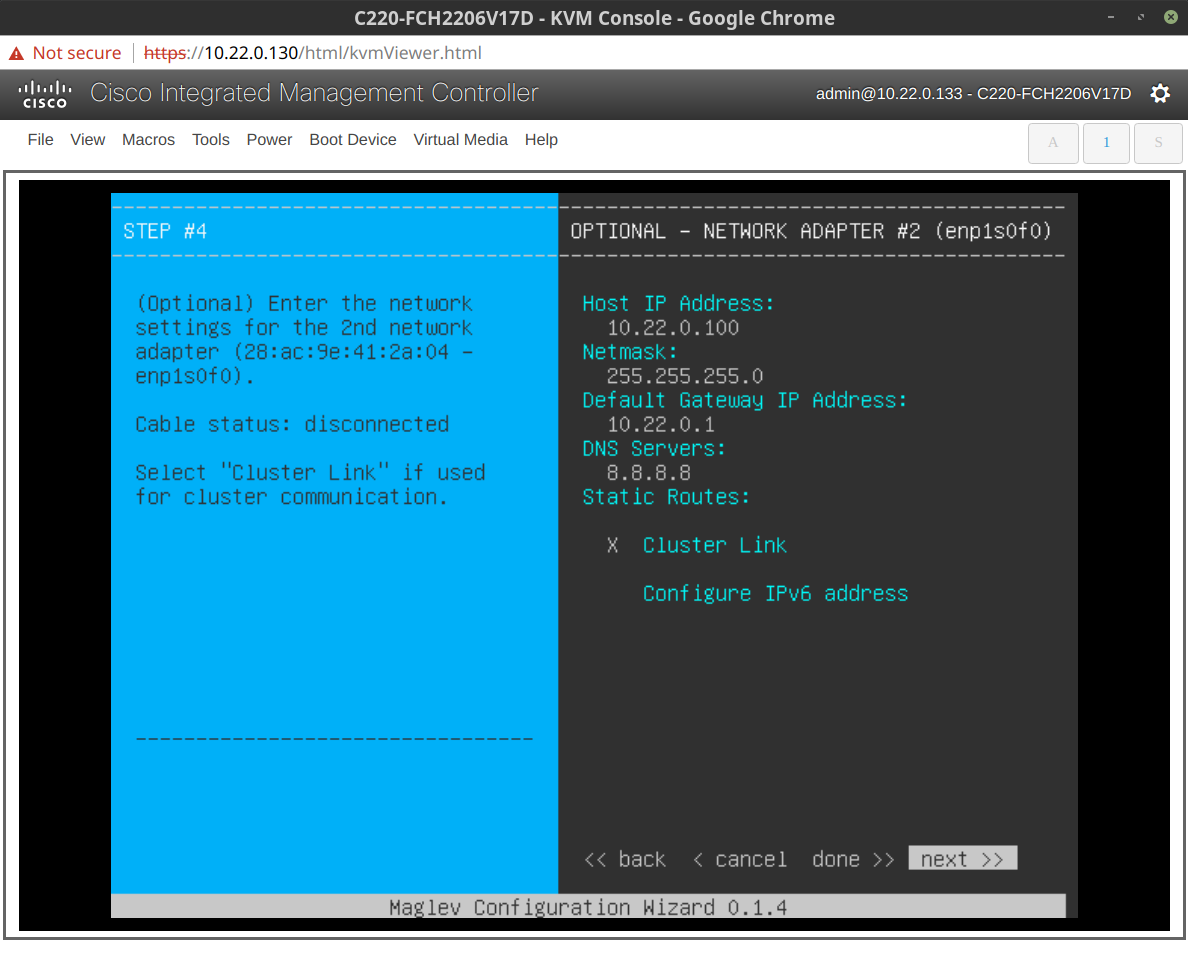
\includegraphics[height=9cm]{img/sc_002.png}
	\caption{DNA Center Configuration Wizard - Entering Management IP}
	\label{fig:installguide-dna-center-install-step-4}
\end{figure} 

\paragraph{Schritt 5}
~\\
Anschliessend muss die Virtuelle Cluster IP Adresse hinterlegt werden. Da es sich in unserem Fall um eine Standalone Installation handelt, kann dieser Schritt übersprungen werden. 
\begin{figure}[H]
	\centering
	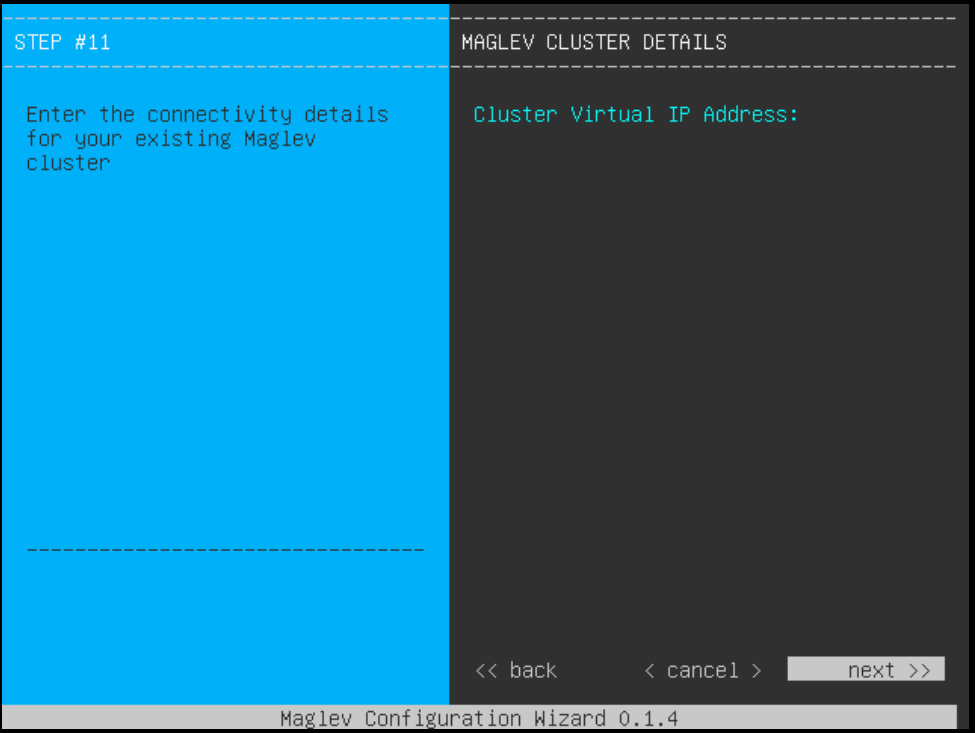
\includegraphics[height=9cm]{img/installguide/installguide-step11.PNG}
	\caption{Cisco - Maglev Configuration Wizard - Cluster Virtual IP Address}
	\label{fig:installguide-dna-center-install-step-11}
\end{figure} 

\paragraph{Schritt 6}
~\\
In diesem Schritt des Wizards werden alle User Account Einstellungen festgelegt. Hierbei ist zu beachten, dass das "Linux Password" für den SSH Zugriff benötigt wird und die "Administrator Passphrase" für den Zugang zum Web Interface. Klicken Sie anschliessend auf \textit{next}.

\begin{figure}[H]
	\centering
	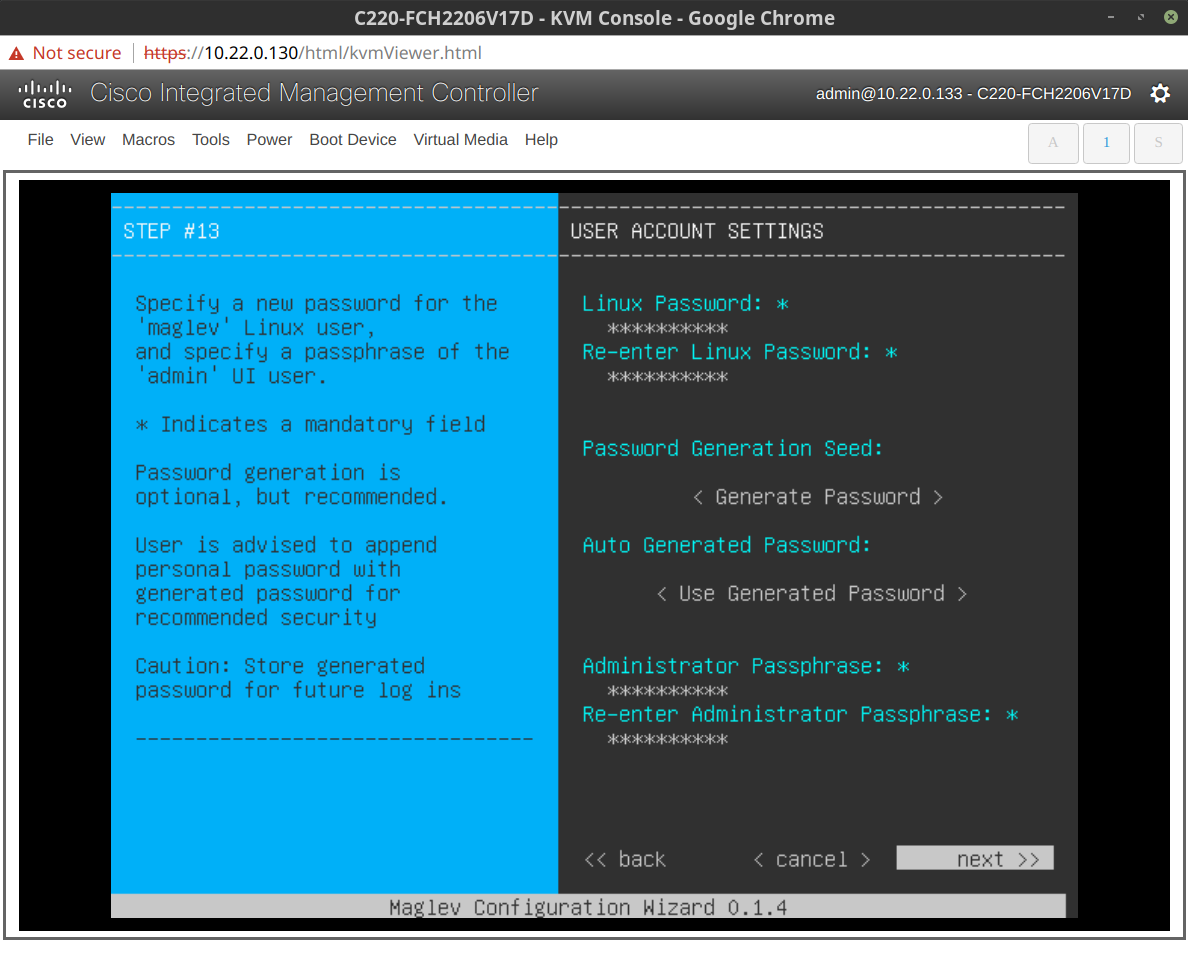
\includegraphics[height=9cm]{img/sc_003.png}
	\caption{DNA Center Configuration Wizard - Entering Authentification Data}
	\label{fig:installguide-dna-center-install-step-13}
\end{figure}

\paragraph{Schritt 7}
~\\
In diesem Schritt wird der gewünschte NTP Server eingegeben. In unserem Fall \url{pool.ntp.org}.
\begin{figure}[H]
	\centering
	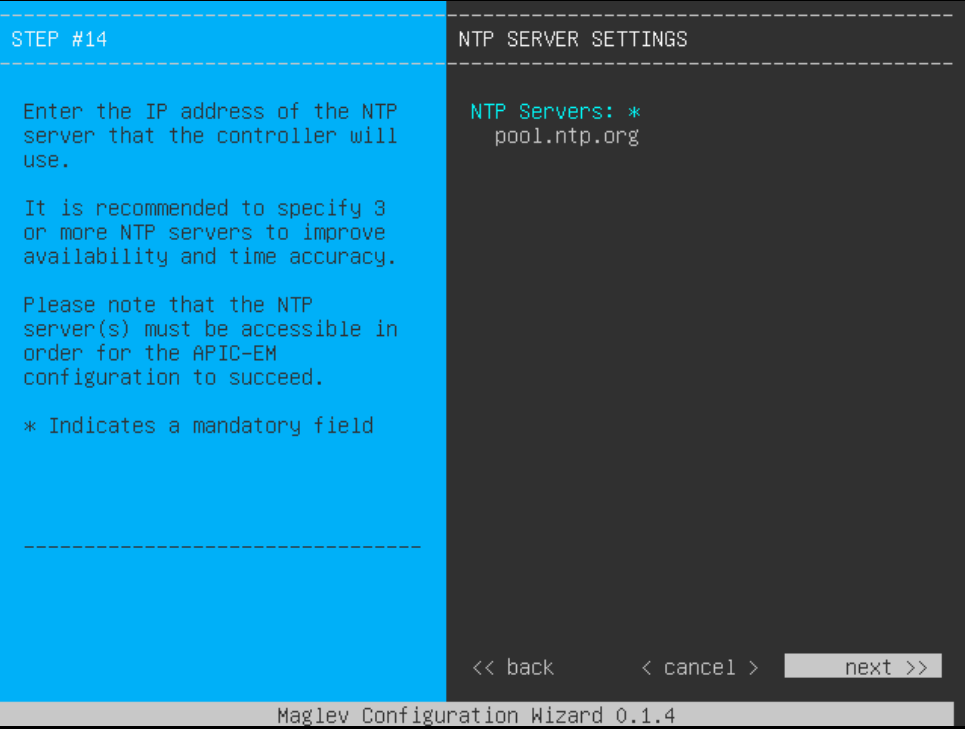
\includegraphics[height=9cm]{img/installguide/installguide-step14.PNG}
	\caption{Cisco - Maglev Configuration Wizard - NTP Server}
	\label{fig:installguide-dna-center-install-step-14}
\end{figure} 

\paragraph{Schritt 8}
~\\
Das DNA Center benötigt für das interne Netzwerk ein Subnet. Geben Sie das entsprechende Subnet ein.
\begin{figure}[H]
	\centering
	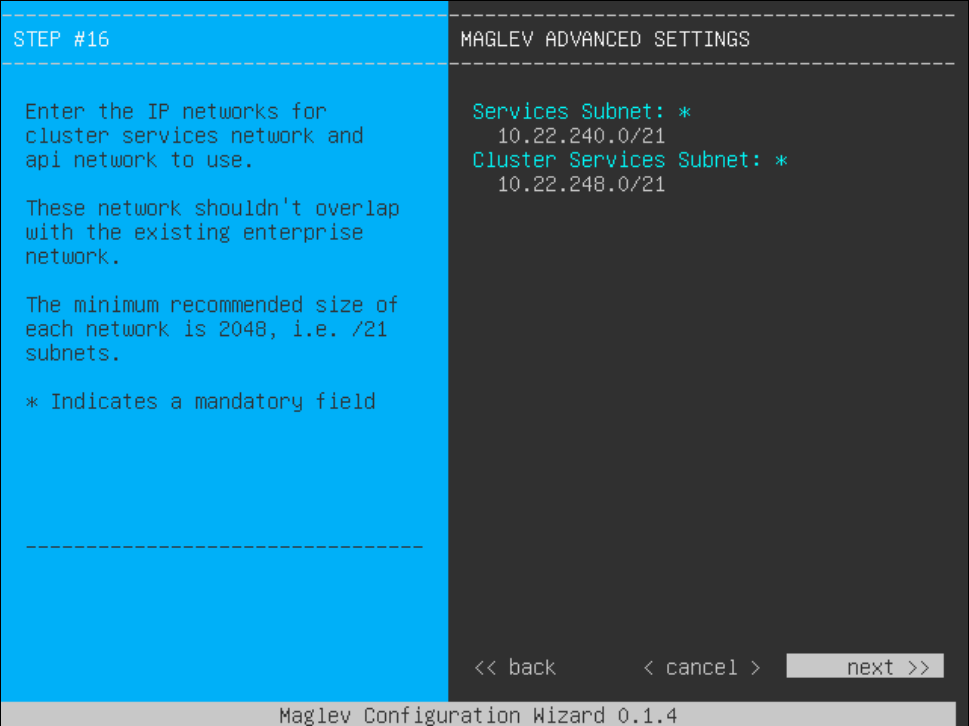
\includegraphics[height=9cm]{img/installguide/installguide-step16.PNG}
	\caption{Cisco - Maglev Configuration Wizard - Service Subnet}
	\label{fig:installguide-dna-center-install-step-16}
\end{figure} 

\paragraph{Schritt 9}
~\\
Schliessen Sie den Wizard ab in dem Sie im Dialog entweder \textit{next} oder \textit{proceed} anwählen.

\paragraph{Schritt 10}
~\\
Nun wird das DNA Center aufgesetzt. Dieser Prozess dauert mehrere Stunden. 

\begin{figure}[H]
	\centering
	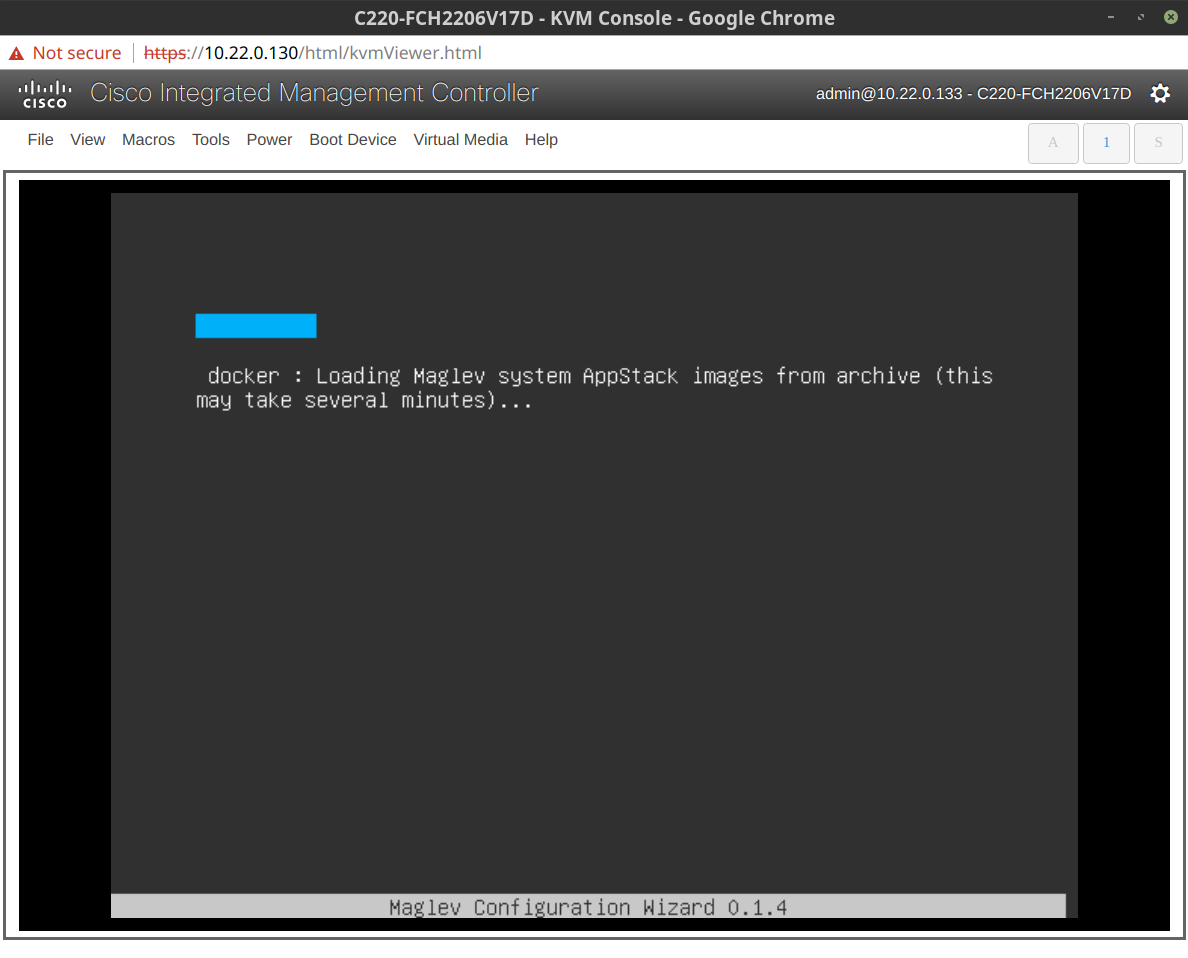
\includegraphics[height=9cm]{img/sc_004.png}
	\caption{DNA Center Configuration Wizard - DNA Center uses docker}
	\label{fig:dna-center-install-step-install}
\end{figure}

\subsection{Einloggen in Web GUI}
Nachdem der \textit{Maglev Configuration Wizard} die Installation angeschlossen hat, kann das DNA Center über das Webinterface aufgerufen werden.

Dazu wird mit einem gängigen Webbrowser die entsprechende Url aufgerufen. In unserem Fall \url{https://10.22.0.100}.

Anschliessend erfolgt das Login mit den im vorhergehenden Schritt definierten Anmeldedaten. 

\begin{figure}[H]
	\centering
	\includegraphics[height=9cm]{img/sc_005.png}
	\caption{DNA Center Web GUI - Login Seite im Webbrowser}
	\label{fig:installguide-dna-center-gui-1}
\end{figure}

\subsection{Cisco Credentials}
Gleich zu Beginn verlangt das DNA Center die Cisco Credentials die mit dem Smart Account verknüpft sind, in welchem die Lizenzen verwaltet werden. Diese Informationen können auch zu einem späteren Zeitpunkt noch eingetragen werden.
\begin{figure}[H]
	\centering
	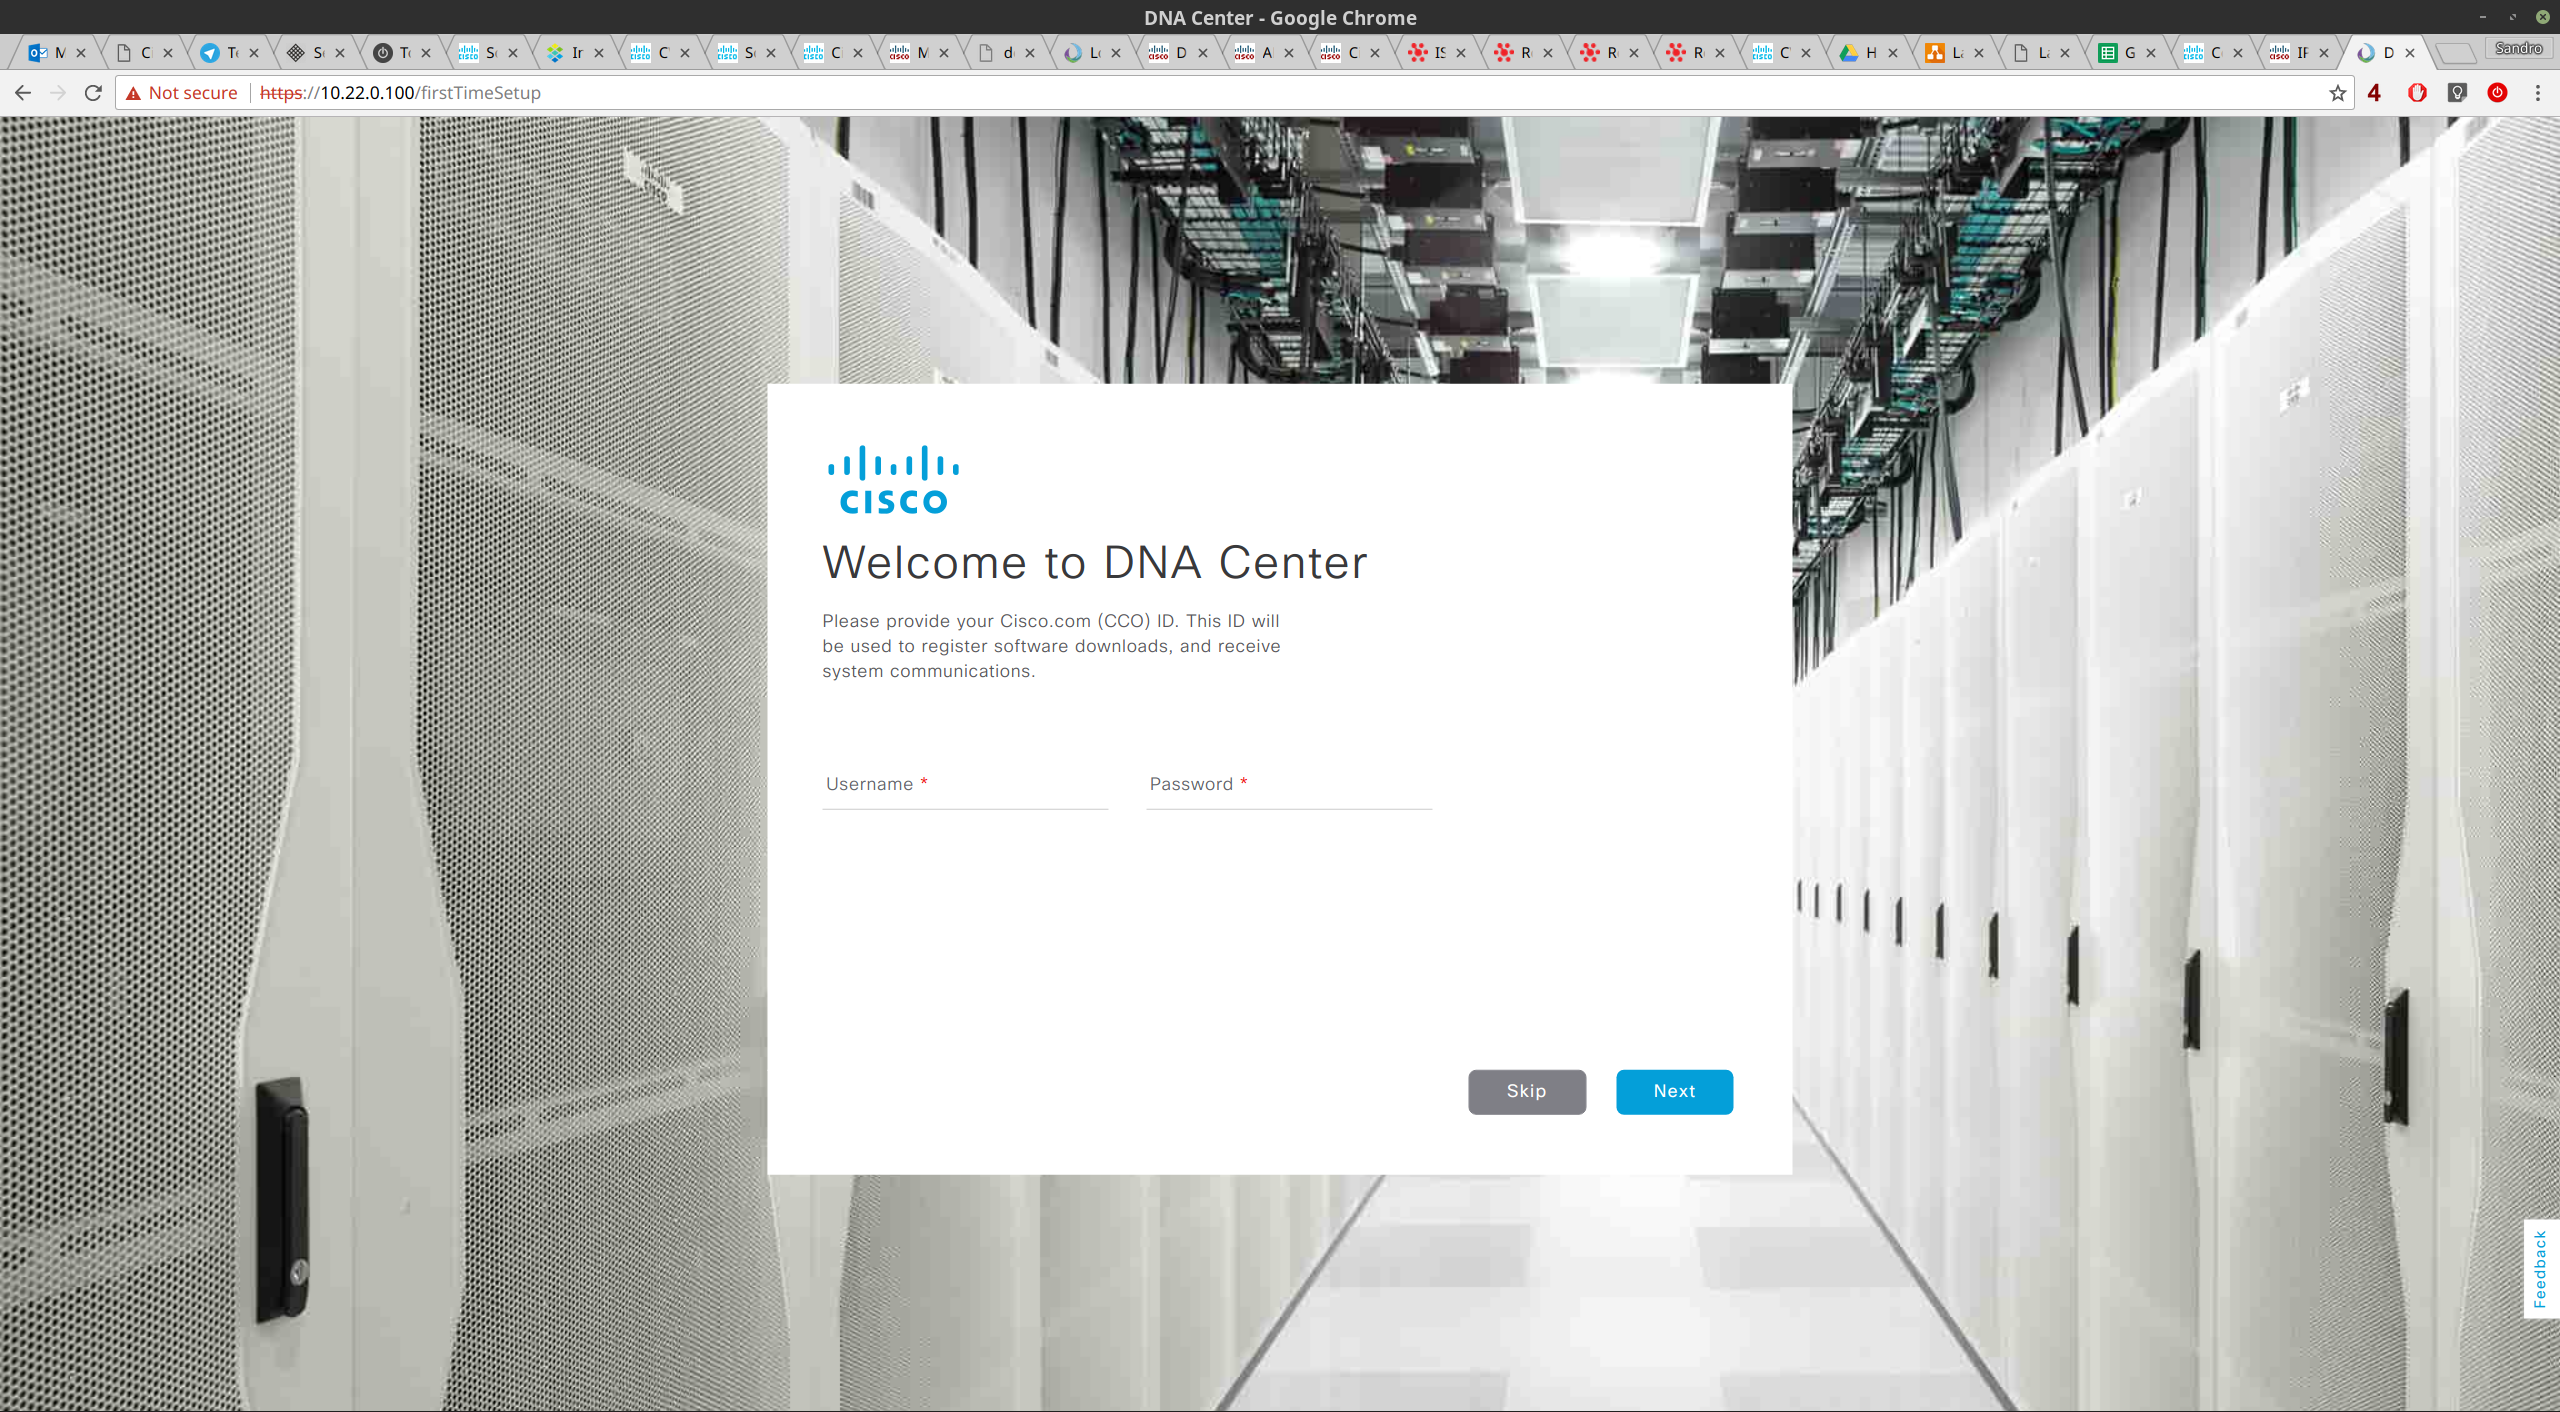
\includegraphics[height=9cm]{img/sc_006.png}
	\caption{DNA Center Web GUI - Cisco Credentials for Licences}
	\label{fig:installguide-dna-center-gui-2}
\end{figure}

\subsection{IP Address Manager - IPAM Server}

Im nächsten Schritt kann ein IPAM Server angegeben werden. Diese Einstellung kann ebenfalls später angepasst werden, weshalb wir diesen Schritt zu Beginn übersprungen haben. In unserem Fall haben wir den Infoblox Server mit der Addresse \url{10.22.0.21} eingegeben. 

\begin{figure}[H]
	\centering
	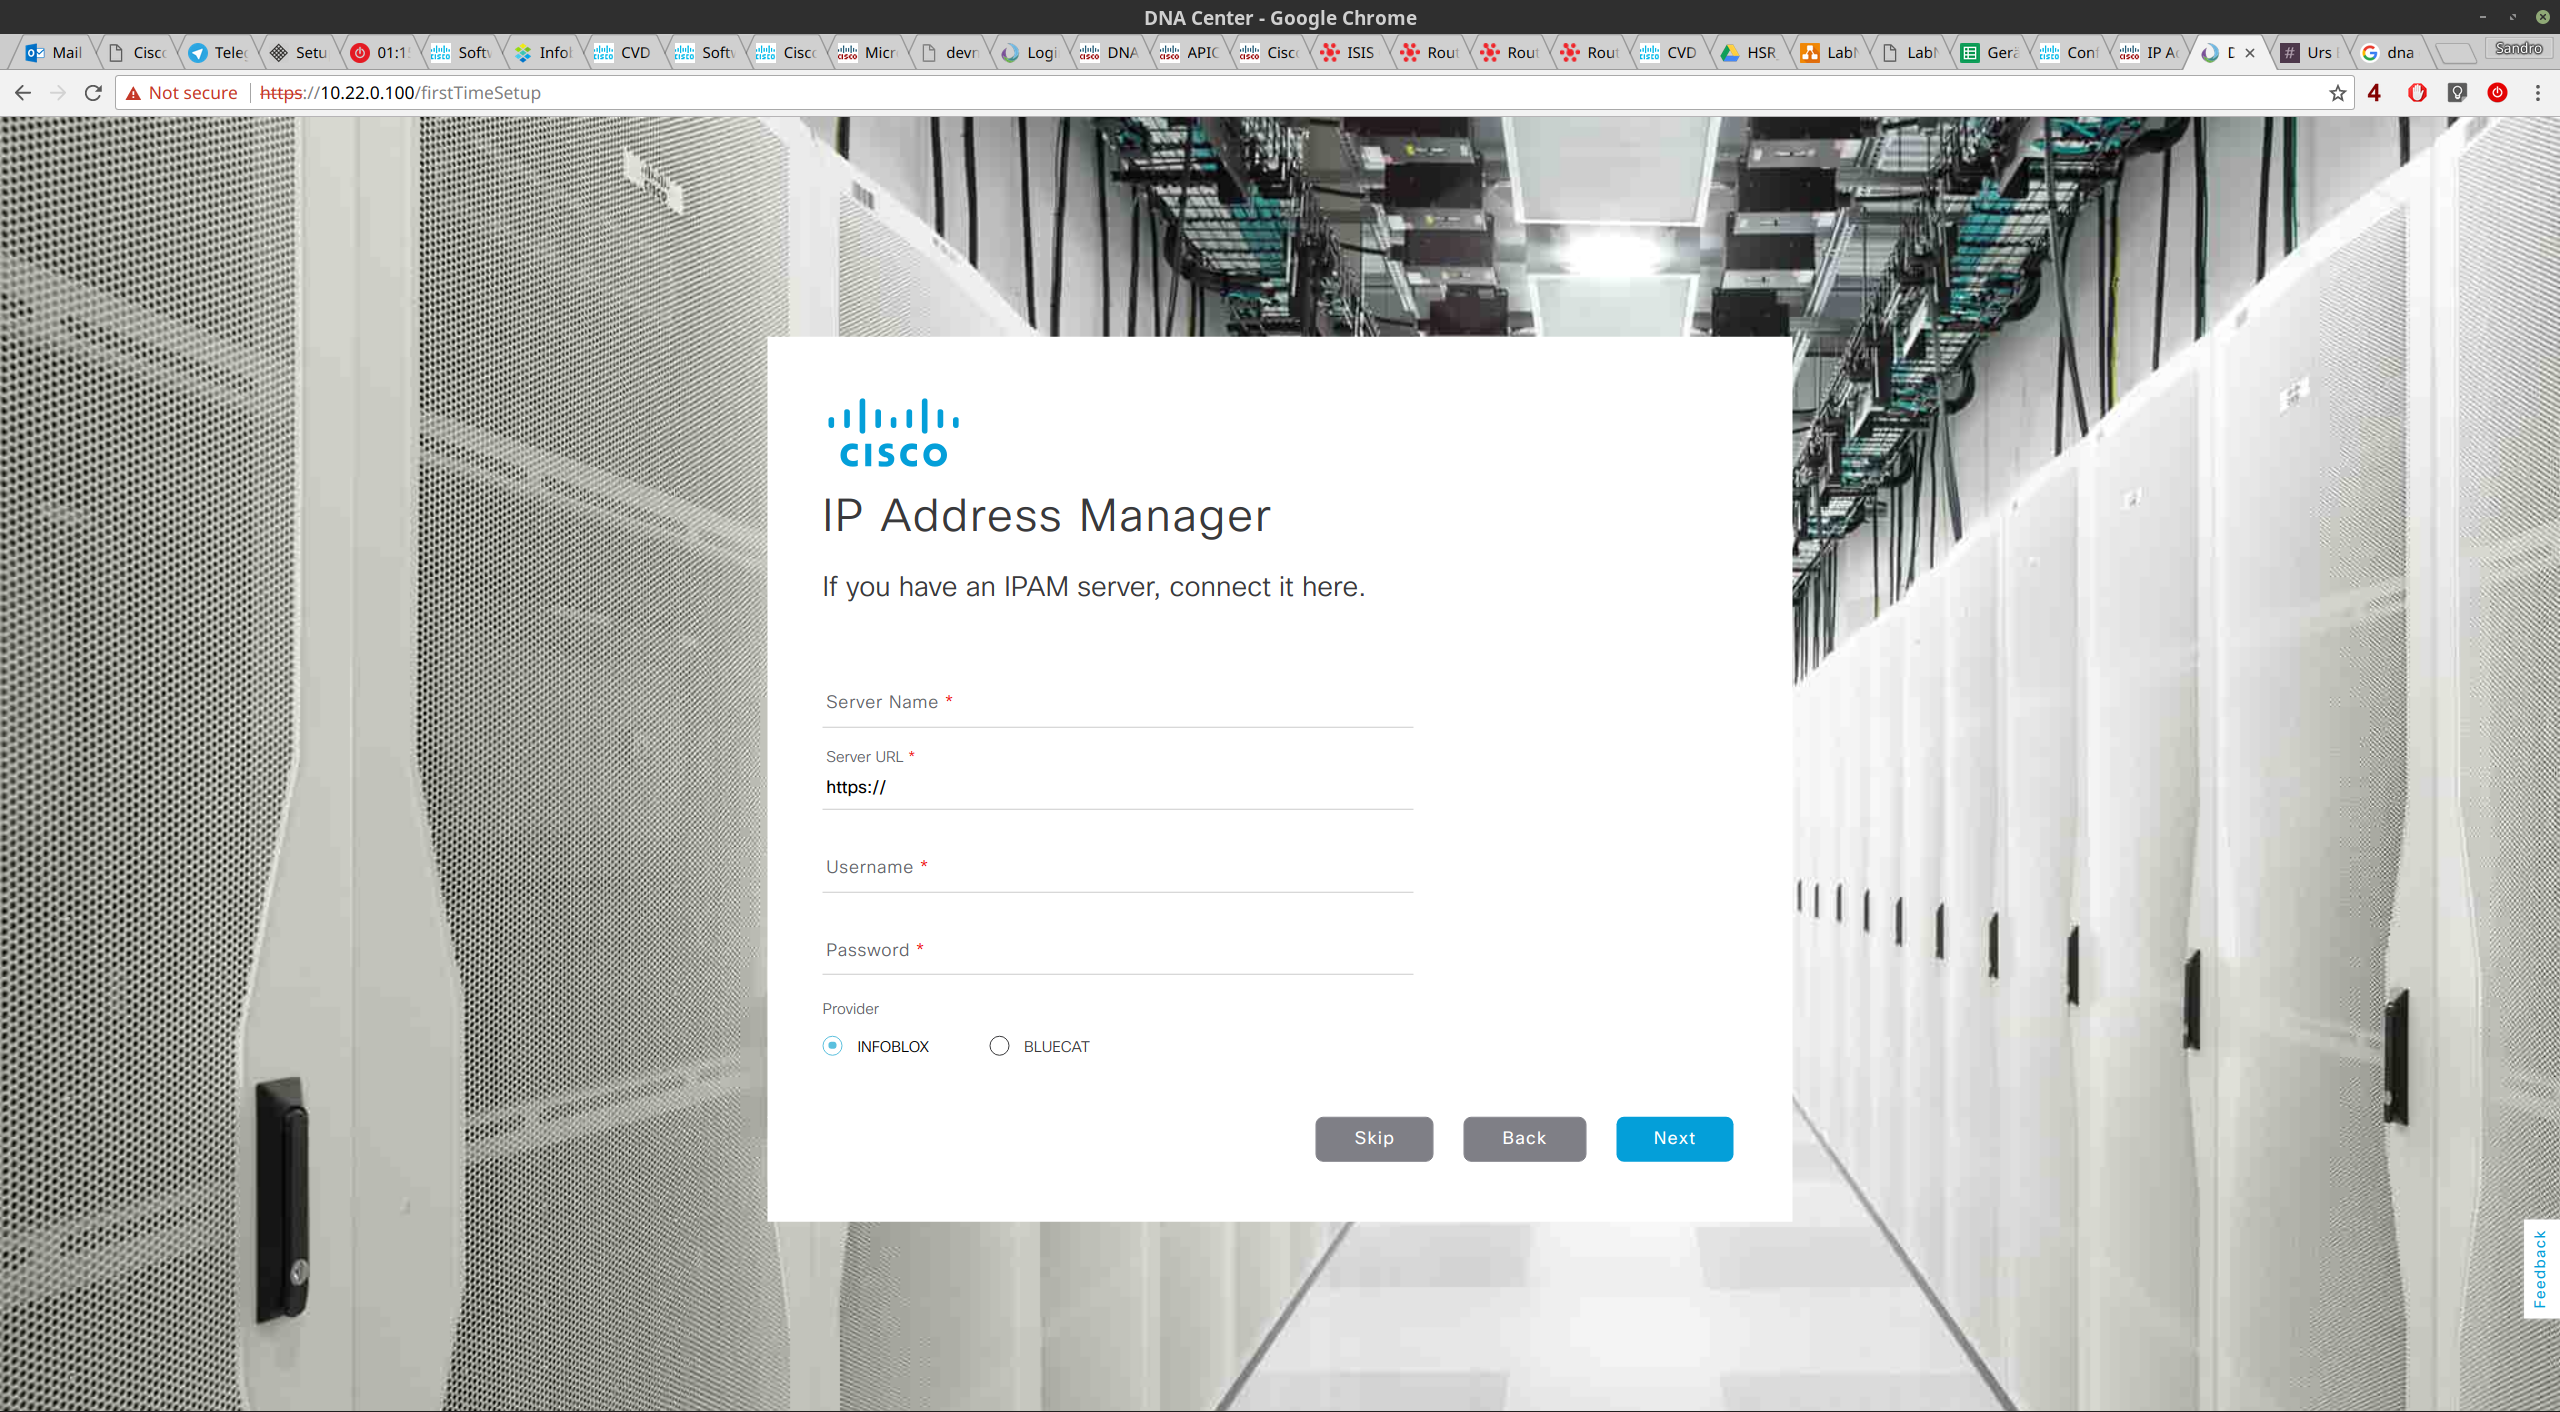
\includegraphics[height=9cm]{img/sc_007.png}
	\caption{DNA Center Web GUI - Cisco IPAM - Enter Infoblox Credentials}
	\label{fig:installguide-dna-center-gui-3}
\end{figure}

\subsection{Terms and Conditions}
Im folgenden Abschnitt sind das \textit{Cisco End User Licence Agreement (EULA)} und alle weiteren relevanten \textit{Terms} aufmerksam zu lesen und mit \textit{Next} zu akzeptieren. 

\begin{figure}[H]
	\centering
	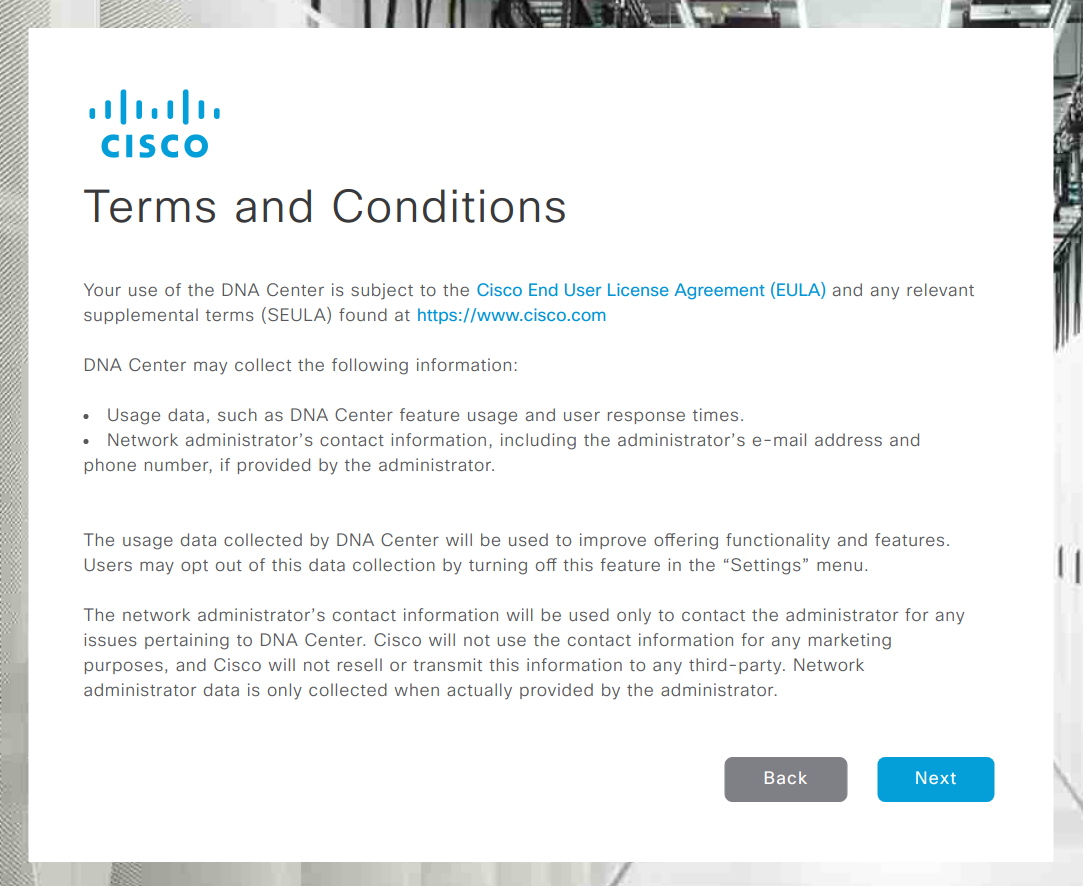
\includegraphics[height=7cm]{img/installguide/webgui-termsandcondition.png}
	\caption{DNA Center Web GUI - Terms and Conditions}
	\label{fig:installguide-dna-center-gui-4}
\end{figure}

\subsection{Abschluss}
Danach ist die initiale Konfiguration beendet und das DNA Center Dashboard wird angezeigt.

\begin{figure}[H]
	\centering
	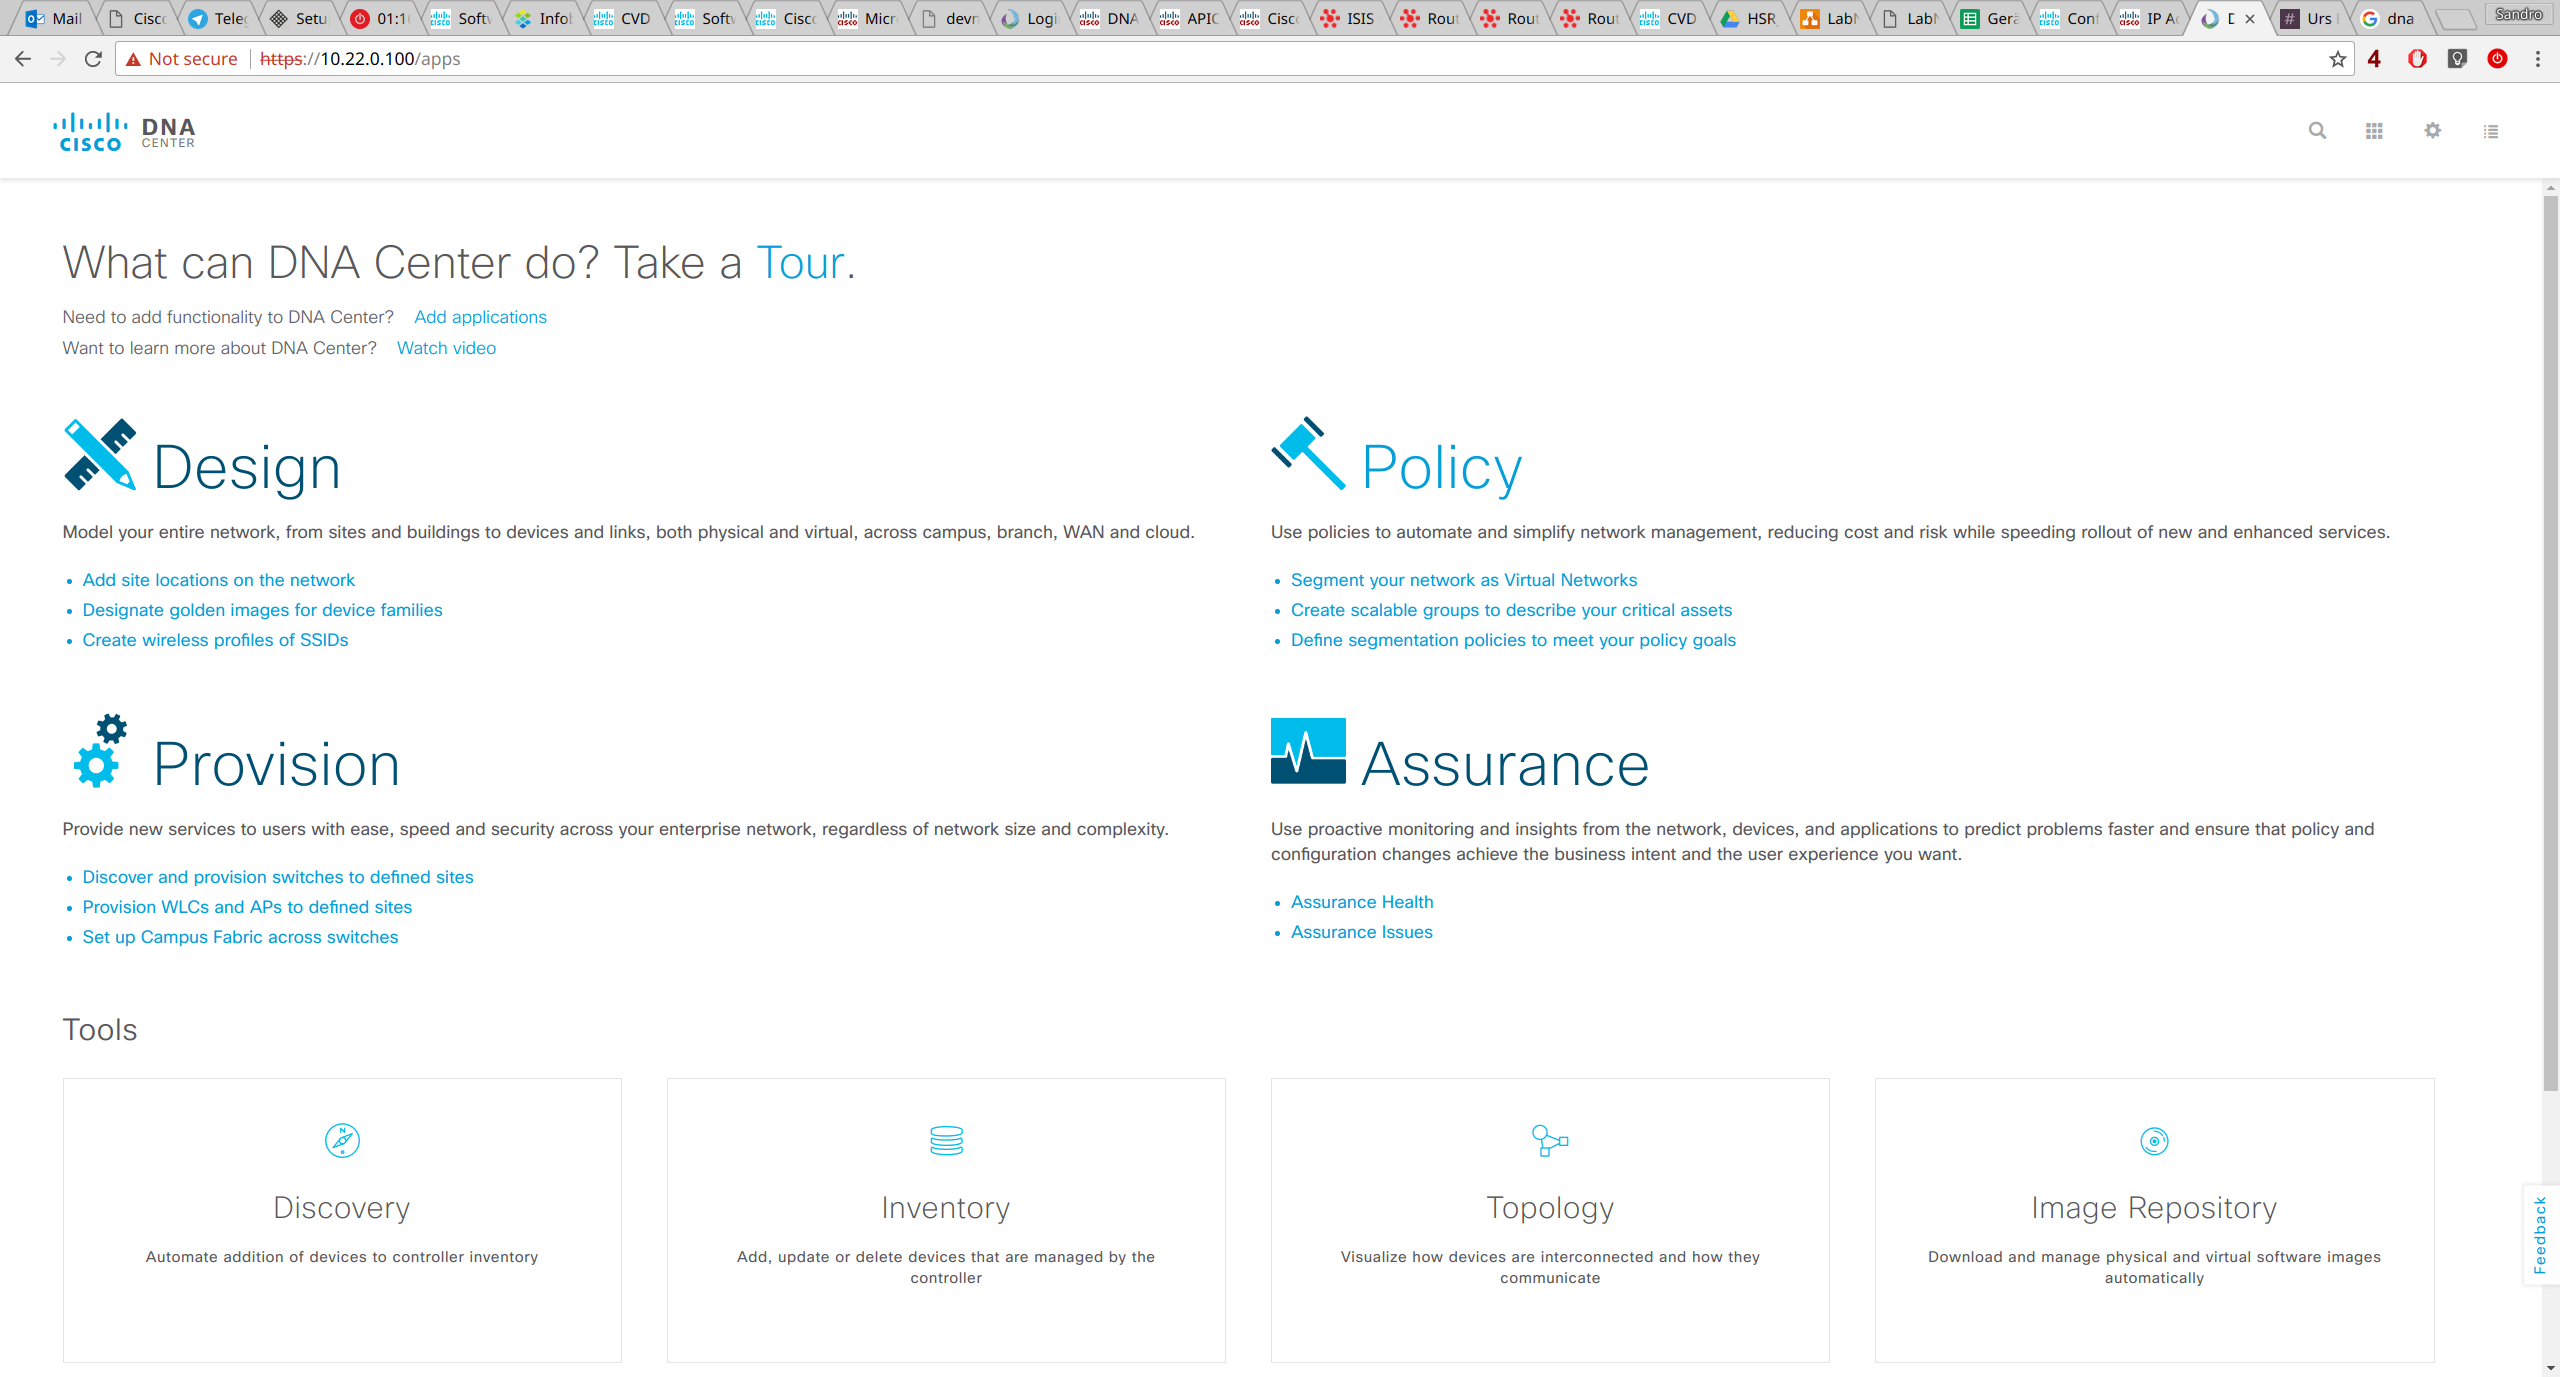
\includegraphics[height=9cm]{img/sc_008.png}
	\caption{DNA Center Web GUI - Dashboard}
	\label{fig:installguide-dna-center-gui-5}
\end{figure}

\subsection{ISE Integration}
Nebst dem Infoblox muss auch noch der Cisco ISE integriert werden. Es gilt dabei zu beachten, dass der Cisco ISE in der richtigen Version vorliegen muss. In unserem Falle \textbf{2.3.0.298}.
Damit eine Verknüpfung zwischen dem Cisco DNA Center und dem Cisco ISE hergestellt werden kann, müssen im Cisco ISE zuerst einige Einstellungen vorgenommen werden. 
Alle diese Schritte sind dieser Anleitung (Siehe: \cite{cisco-dna-appliance-installation-guide-release-1-chapter-post-installation-task}) entnommen worden.

\subsubsection{ISE Vorbereiten}

\begin{enumerate}
	\item In Cisco ISE einloggen.
	\item \textit{Administration $\rightarrow$ Deployment} auswählen.
	\item Gewünschten ISE node auswählen und in der Nachfolgenden Ansicht. \textit{Enable SXP Service}, \textit{Enable Passive Identity Service} und \textit{pxGrid} mit einem Haken anwählen. 
	\item Speichern drücken.
	\item Im \textit{Profiling Configuration} Tab muss mindestens \textit{RADIUS} und \textit{SNMPQUERY} ausgewählt sein. 
	\item Unter \textit{Administration $\rightarrow$ Settings $\rightarrow$ ERS Settings} \textit{Enable ERS for Read/Write} auswählen und mit \textbf{OK} bestätigen. 
\end{enumerate}

\subsubsection{Cisco ISE im DNA Center hinterlegen}
\begin{enumerate}
	\item In Cisco DNA Center Web GUI einloggen.
	\item System Settings auswählen (Zahnrad oben rechts).
	\item Cisco ISE Panel auswählen.
	\item \textit{Configure Setting} wählen.
	\item Unter \textit{Settings- Auhentication and Policy Servers} auf das grosse Plus (+) drücken. 
	\item Im neuen Dialog Management IP Adresse, Shared Secret, Username, Password, FQDN und  Subscriber Name eingeben. 
	\item Update wählen. 
\end{enumerate}

\begin{figure}[H]
	\centering
	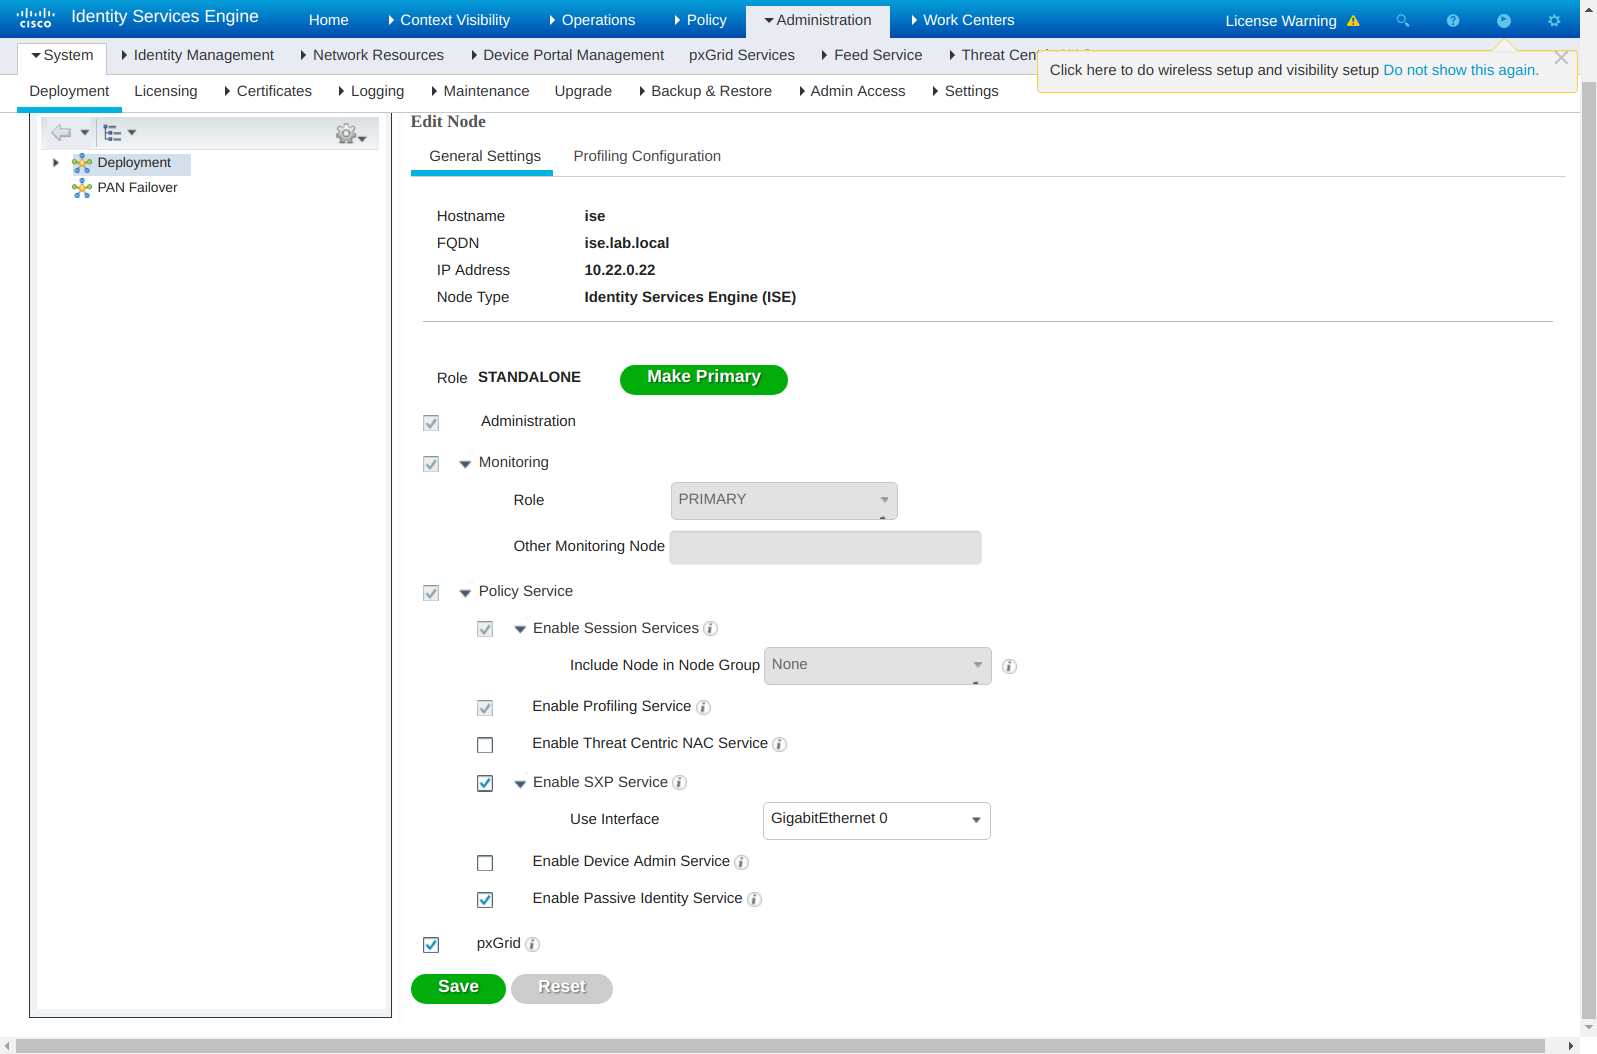
\includegraphics[height=9cm]{img/installguide/cisco-ise.png}
	\caption{Cisco ISE benötigte Konfigurationen für die DNA Center Verknüpfung}
	\label{fig:installguide-cisco-ise}
\end{figure}

